\chapter{Concept}
\label{Concept}

This chapter covers the conceptual design of the navigation and defines requirements for some its parts.\\

Based on the analysis in chapter \ref{relatedwork} the navigation stack seems to be a well fitting core structure for the navigation. The use case leads to modifications to the recommended setup pictured in Figure \ref{navigation stack setup}.

Afterwards the tasks of the nodes in move\_base need to be defined. These will be categorized into the global and local stage, each consisting out of a planner and a costmap.
Additionally the setup requires a nodes, that autonomously find new goals for the navigation and transform the sensor data into a usable format. 

\section{Sensor transforms}
To know the position of every sensor relative to the robot and its odometry the tf\_tree has to be build. While this can be realized using static transform publishers, there is also a cleaner way using the ROS package robot\_state\_publisher. This requires a robot description in URDF format that specifies the relations between everything mounted on the robot.\\

The required odom frame is build by using the position derived from the wheel encoder data.

\section{Map}

The map is a representation of the robots environment. If this is known from the start it is clear, where the robot can go and where not.\\

Like described amcl and the map—server are not suited for this use case.

A SLAM (simultaneous localization and mapping) algorithm becomes highly useful since the robot might drive multiple rounds, allowing the robot to build its own map. This potentially allows a goal extraction from the map instead of estimating it by using the sensor data stream.

This node will publish the transform between the map and the odom frame, so the position of the robot and every sensor signal can be determined relative to the environment.\\

Unfortunately the data that can be fed to the SLAM algorithm is very limited, since it is not guaranteed, that the lidar all ways sees static obstacles. Another data source for the SLAM algorithm could be the points extracted from the roadDetection. Unfortunately the road markings are similar to a corridor and do not have a lot of features, other than their curvature.\\

This significantly decreases the reliability of the map which therefore will highly depend on good odometry.

To get the best map, both of the data inputs have to be used, which results in the need of a SLAM algorithm with multiple inputs.\\


\subsection{Global stage}
The general task of the global planner is like described in the theoretical background to plan a rough path through the grid of the costmap, that does not collide with any lethal cell.\\

In this scenario the global planner will be required to guide the robot on the correct lane as well. This results in the following requirements:

\begin{itemize}
	\item The global costmap needs information about the road markings and the obstacles detected by the lidar scan
	\item The global costmap needs to incorporate cost that generate a preference for the right lane, but allow the global path to go to the left in case of an obstacle
	\item The global planner has to respect not only lethal but every cost
\end{itemize}

\subsection{Local stage}
The local stage on the other hand has the task of finding a path, that is feasible for the dynamics of the robot, that does not collide with objects.\\
This path is supposed to be close to the global path and follow its lane changes, but it needs to be able to separate itself from it, if necessary.

Therefore the local costmap needs to have information about the road markings and the obstacles detected by the lidar scan.

\section{PoseFinder}
The job of this node is to extract a goal from the sensor data or the map (if available).\\

The roadDetection is only able to detect the road to a certain distance, further away the course of the road is unknown.\\
To allow the planners to generate smooth paths the distance, at which goals need to be found should be relatively far away. Therefore this node needs to estimate the upcoming course and repeatably send new goals, since it is uncertain, if the goal is actually on the road or not.

If a map is available the estimation is redundant, since the map is likely to be more precise.
\section{Sensor filter}

This block incorporates the nodes that process the sensor data into a usable format, that is usable for the navigation\_stack. 
Therefore it consists out of the following nodes:

\begin{itemize}
	\item \textbf{roadDetection} will extract approximated polynomials for the road markings and the lanes from the camera data
	\item \textbf{markfreespace} needs to publish point clouds to the costmaps and the SLAM algorithm consisting out of the roadDetection data and the lidar scan.
\end{itemize}

Like described in the requirement the simulator is supposed to produce realistic sensor data, which might needs filtering, these filters are additionally located in this block.

\section{Resulting concept}
The following simplified schematic is the concept of the navigation stack setup. Not all of the connections between the nodes will be highlighted, to keep the schematic simple.\\

\begin{figure}[H]
	\begin{center}
		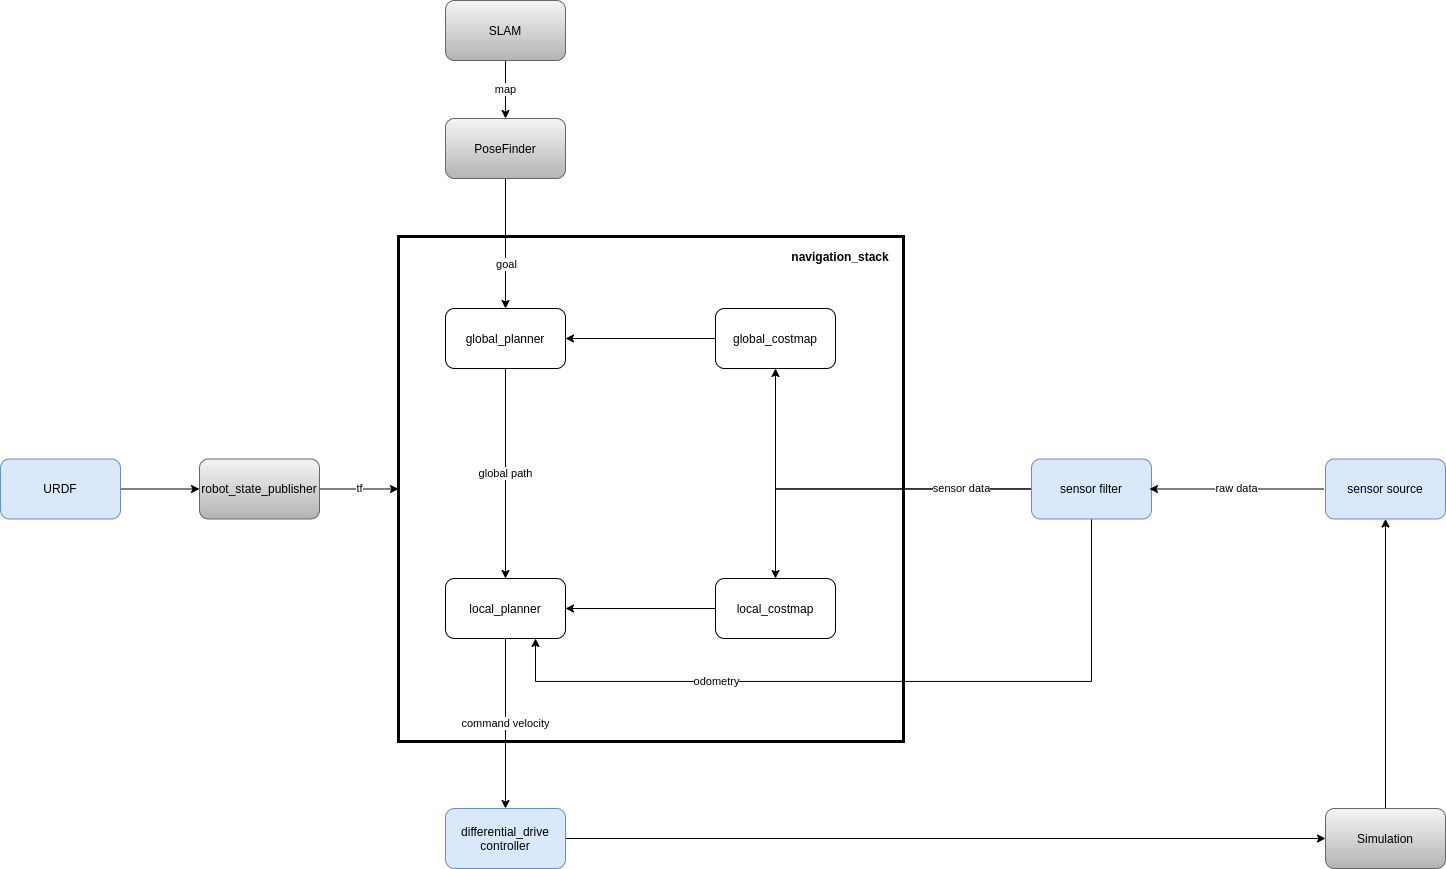
\includegraphics[width=140mm]{Pictures/Updated navigation concept}
		\caption[updated navigation concept]{Updated navigation concept}
	\end{center}
\end{figure}



The PoseFinder will find repeatedly find goals based on the current state of the map and the sensor data and sends it to the navigation stack. This uses the filtered sensor data to determine, where the robot is, where it is allowed to go and where not. The cascading planners then produce first a rough, collision free, path on the correct lane and then a path that is possible for the dynamics of the robot. This path then gets converted to velocity commands and sent to the differential drive controller.\\




